\documentclass[xcolor=dvipsnames,hyperref={pdfpagelabels=false}]{beamer}

\usetheme{Boadilla}

\newcommand{\bi}{\begin{itemize}}
\newcommand{\ei}{\end{itemize}}
\newcommand{\be}{\begin{enumerate}}
\newcommand{\ee}{\end{enumerate}}
\newcommand{\bc}{\begin{center}}
\newcommand{\ec}{\end{center}}
\newcommand{\bd}{\begin{description}}
\newcommand{\ed}{\end{description}}
\newcommand{\I}{\item}
\newcommand{\f}{\frame}
\newcommand{\ft}{\frametitle}

\title{Offline Software Overview}
\subtitle{GlueX Collaboration Meeting}
\author[Mark Ito]{Mark M.\ Ito}
\date{February 19, 2015}
\institute[JLab]{Jefferson Lab}

\begin{document}

\f{\titlepage}

\f{\ft{Outline}
\be
\I Software Review III
\I Version Management System
\I Run Conditions Databases
\I Commissioning-Branch-to-Trunk Migration
\I Miscellaneous Topics
\I Summary
\ee
}

\f{\ft{Software Review III}
\bc
See Curtis's talk in Business Session (Saturday)
\ec
}

\f{\ft{Version Management System}
\bi
\I Goals:
  \be
  \I Communicate a consistent set of versions.
    \bi
    \I Identify working combinations
    \I Coordinate collaborative work
    \ei
  \I Specify a set of versions to be built.
    \bi
    \I Green-field builds
    \I Adding versions to existing build trees
    \ei
  \I Set-up environment to use specific versions.
    \bi
    \I Ensure consistency with desired set of versions.
    \ei
  \ee
\I Implemented with a single XML file and some Perl scripts
\I Part of build\_scripts
\ei
}

\f{\ft{Run Conditions Databases}
\bi
\I Two of them:
  \be
  \I Data Monitoring
    \bi
    \I Developer: Sean
    \I Used to drive offline monitoring
    \ei
  \I RCDB
    \bi
    \I Developer: Dmitry
    \I Direct input from Run Control
    \ei
  \ee
\I Plan: combine best of both
\ei
}

\f{\ft{Data Monitoring}
$$
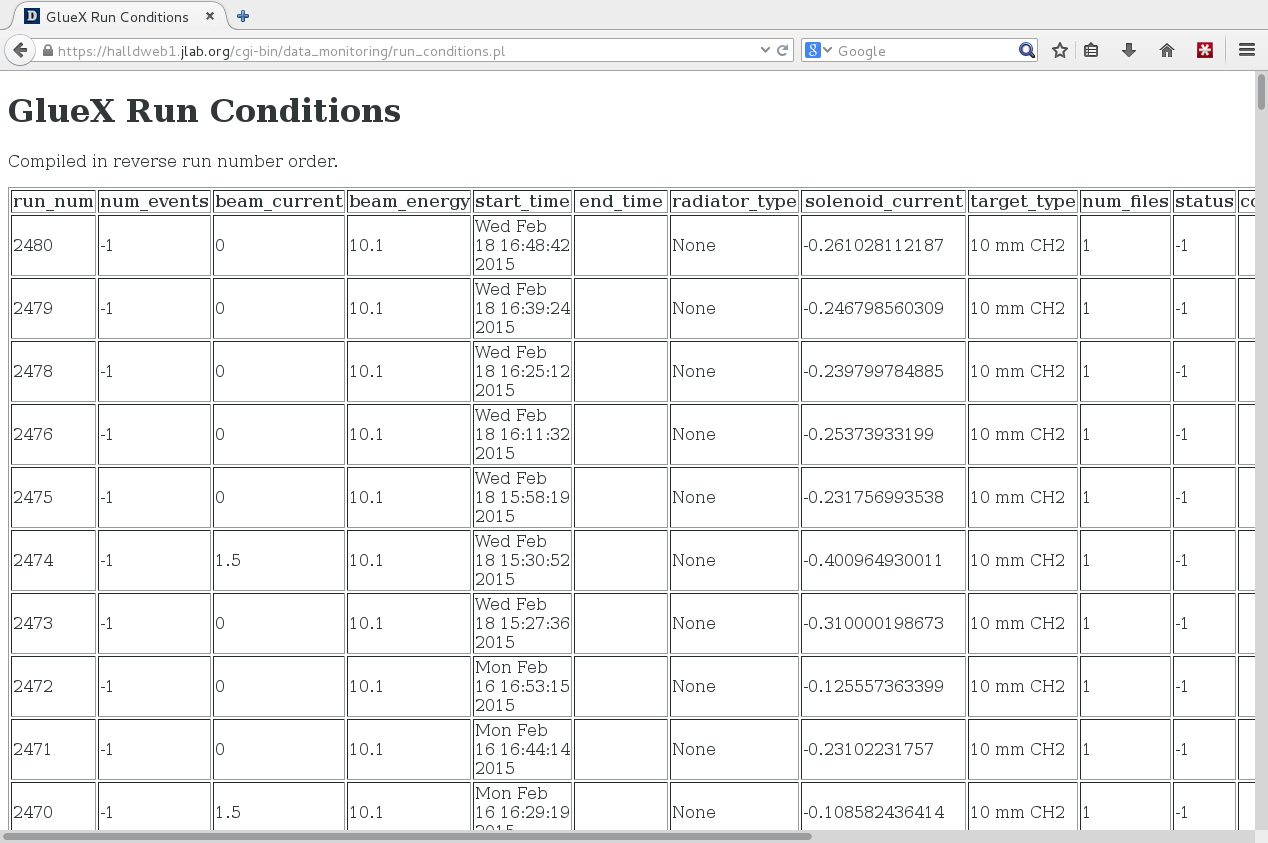
\includegraphics[width=4.3in]{data_monitoring.png}
$$
}

\f{\ft{RCDB}
$$
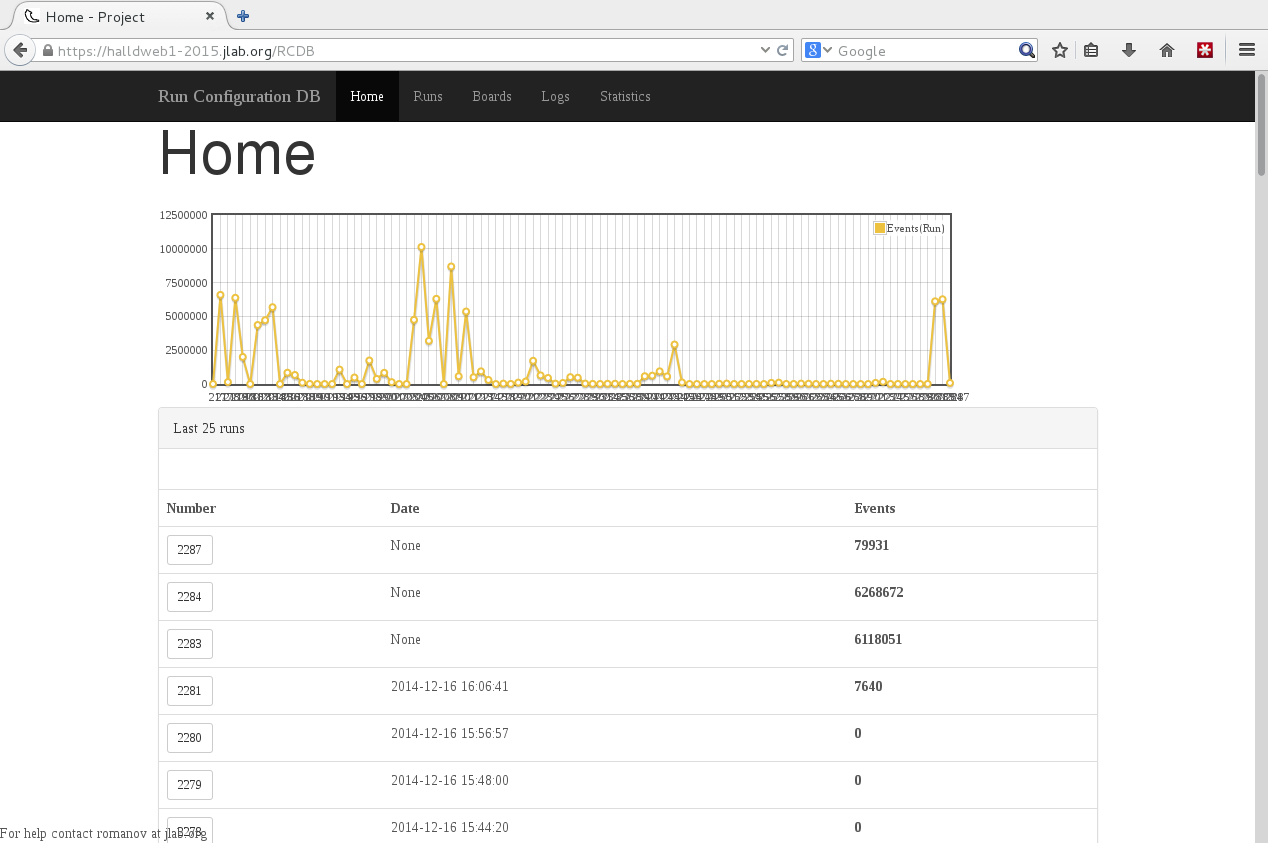
\includegraphics[width=4.3in]{rcdb.png}
$$
}

\f{\ft{Commissioning-Branch-to-Trunk Migration}
\bi
\I During Fall run, most development done on ``branches/sim-recon-commissioning''
\I Trunk largely dormant after some early confusion
\I Merging changes branch-to-trunk has proved difficult
\I Current focus: fix the commissioning branch
  \bi
  \I Simulated data not getting reconstructed properly
  \ei
\I Q/A checks were only run on trunk
\ei
}

\f{\ft{Miscellaneous Topics I}
\bi
\I EVIO support in Public Builds (gluex\_install)
\I Sean implemented system dependent time cuts when converting simulated HDDM data to EVIO. (Use the ``mc'' variation)
\I Commissioning Simulations
  \bi
  \I Several iterations tried
  \I Rates roughly consistent with reality
  \I normalization worked out for incoherent bremsstrahlung beam
  \ei
\I Richard implements change to allow association of photons with showers in the calorimeters.
\I GlueX Project Accounts for JLab Farm: gxproj1, gxproj2, and gxproj3
\I Now able to extract physics signals from REST data (our DST format, Justin)
\ei
}

\f{\ft{Miscellaneous Topics II}
\bi
\I Data Challenge 3: preparations still grinding forward
\I Meeting with JLab SciComp on farm features (see talk later in this session)
\I New scheme for getting the magnetic field into JANA using CCDB and Resources (Sean)
  \bi
  \I run-dependent look-up of correct field map
  \ei
\I EventStore: Sean has done a lot of work recently.
  \bi
  \I DB creation and management scripts in Subversion, documentation under way
  \I eventstore plugin designed, implementation/documentation under way
  \ei
\ei
}

\f{\ft{Summary}
\bi
\I Reconstruction performed well during Fall run.
\I Software Review III went well.
\I Source code management needs to get more formal. (See dead trunk problem above.\footnote{Shel Silverstein. ``The Giving Tree.'' Harper \& Row. New York (1964).})
\I Testing regime needs expansion
  \bi
  \I profiling
  \I tests with real data
  \I unit testing?
  \ei
\ei
}

\end{document}

